% !TEX root = master_thesis.tex
\chapter{Extraction of the beam asymmetries $\Sigma_{\eta}$ and $\Sigma_{\eta'}$}
The beam asymmetry $\Sigma$ is observable when a linearly polarized photon beam and unpolarized liquid hydrogen target are employed. The polarized cross section $\frac{\text{d}\sigma}{\text{d}\Omega}_\text{pol}$ is not symmetric in the azimuthal angle $\phi$ anymore as opposed to the unpolarized cross section $\frac{\text{d}\sigma}{\text{d}\Omega}_0$. It is rather modulated by a cosine dependence which scales with the polarization observable $\Sigma$ and the (linear) beam polarization $p_\gamma$, see equation \eqref{eq:asym} \cite{san}.
\begin{equation}
	\frac{\text{d}\sigma}{\text{d}\Omega}_\text{pol}\left(E_\gamma,\cos\theta,\phi\right)=\frac{\text{d}\sigma}{\text{d}\Omega}_0\left(E_\gamma,\cos\theta\right)\cdot\left[1-p_\gamma\Sigma\left(E_\gamma,\cos\theta\right)\cos\left(2\varphi\right)\right]
	\label{eq:asym}
\end{equation}
Since the incident photon beam is polarized, photon momentum $\vec{k}$ and polarization $\vec{\epsilon}$ span a plane which is referred to as the beam polarization plane. This plane is tilted by the angle $\varphi$ with respect to the reaction plane which is defined by the final state momenta. Naturally, this plane builds the angle $\phi$ in the laboratory system. At the same time the angle of the beam polarization plane in the same reference frame is defined as $\alpha$. It holds 
\begin{equation}
	\varphi=\alpha-\phi.
\end{equation} Figure \ref{fig:angles} illustrates definitions of all angles and planes. 
 \begin{figure}[htbp]
	\centering
	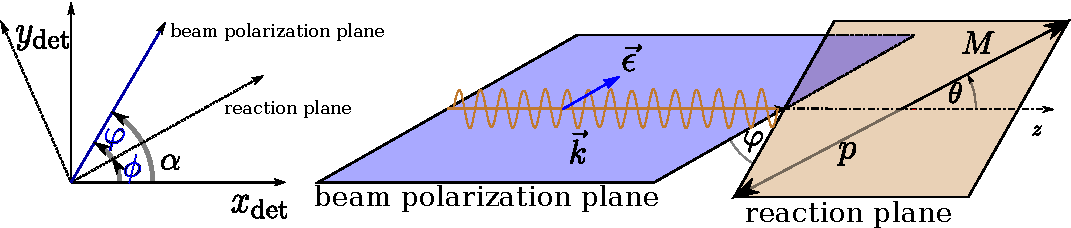
\includegraphics[width=\linewidth]{../DPG2022/figs/angles.pdf}
	\caption{Left: Definition of angles $\alpha,\phi,\varphi$. Right: Photon momentum $\vec{k}$ and polarization  $\vec{\epsilon}$ define the beam polarization plane while the reaction plane is defined by the recoil proton $p$ and produced meson $M$.}
	\label{fig:angles}
\end{figure} 
Theoretically the beam asymmetry can be determined by a measurement of the cross section and a fit using equation \eqref{eq:asym}. However, when calculating polarized cross sections, it is important to have good control over flux normalization and detector acceptance in three dimensions $(E_\gamma,\cos\theta,\phi)$. To avoid this, the measurement of asymmetries can be used to access the polarization observable $\Sigma$ instead. Particularly, data is taken for two distinct orthogonal polarization settings corresponding to $\alpha=\pm\SI{45}{\degree}$.

This chapter will illustrate the process of determining the beam asymmetry for $\eta$ and $\eta'$ photoproduction. The published results of $\Sigma_{\eta}$ \cite{farahphd,eta} are used to check the accuracy and functionality of employed bayesian methods. Bayesian methods, as well as traditional frequentist approaches are used afterwards to extract new results for $\Sigma_{\eta'}$. First, the used methods will be presented and subsequently their application for each final state, respectively.
\section{Methods}
\label{sec:meth}
The beam asymmetry has to be determined via fits to $\phi$ distributions obtained from data. These are performed as either binned or unbinned fits. Both methods allow the application of Bayesian methods as will be discussed in the following. Additionally the advantages and disadvantages off all methods are compared.
\subsection{Event yield asymmetries}
Measurements were made in two distinct polarization settings $\alpha=\pm\SI{45}{\degree}=\alpha^{\bot/\parallel}$. Thus, the polarized cross sections for both settings are given by\footnote{The dependencies of polarized and unpolarized cross sections as well as the beam asymmetry like in equation \eqref{eq:asym} are implied}
\begin{equation}
	\frac{\text{d}\sigma}{\text{d}\Omega}_\text{pol}^\parallel=\frac{\text{d}\sigma}{\text{d}\Omega}_0\cdot\left[1-p_\gamma^\parallel\Sigma\cos\left(2\left(\alpha^\parallel-\phi\right)\right)\right]
	\label{eq:polcs0}
\end{equation}
and 
\begin{align}
	\frac{\text{d}\sigma}{\text{d}\Omega}_\text{pol}^\bot&=\frac{\text{d}\sigma}{\text{d}\Omega}_0\cdot\left[1-p_\gamma^\bot\Sigma\cos\left(2\left(\alpha^\bot-\phi\right)\right)\right]\label{eq:polcs00}\\
	&=\frac{\text{d}\sigma}{\text{d}\Omega}_0\cdot\left[1+p_\gamma^\bot\Sigma\cos\left(2\left(\alpha^\parallel-\phi\right)\right)\right].\label{eq:polcs}
\end{align}
Note that equation \eqref{eq:polcs} holds, because 
\begin{align*}
	\alpha^\bot=\alpha^\parallel+\pi/2 &&\text{and}&&\cos x = -1\cdot\cos(x+\pi).
\end{align*}
Consider now taking the difference of equations \eqref{eq:polcs0} and \eqref{eq:polcs}
\begin{equation}
	\frac{\text{d}\sigma}{\text{d}\Omega}_\text{pol}^\bot-\frac{\text{d}\sigma}{\text{d}\Omega}_\text{pol}^\parallel=\frac{\text{d}\sigma}{\text{d}\Omega}_0\cdot\left(p_\gamma^\bot+p_\gamma^\parallel\right)\Sigma\cos\left(2\left(\alpha^\parallel-\phi\right)\right).
\end{equation}
One can further eliminate the unpolarized cross section from this equation by dividing by the polarization weighted sum of equations \eqref{eq:polcs0} and \eqref{eq:polcs}
\begin{equation}
	\alpha\cdot\frac{\text{d}\sigma}{\text{d}\Omega}_\text{pol}^\parallel+\beta\cdot\frac{\text{d}\sigma}{\text{d}\Omega}_\text{pol}^\bot=\frac{\text{d}\sigma}{\text{d}\Omega}_0\cdot\left[\alpha+\beta-\left(\alpha p_\gamma^\parallel-\beta p_\gamma^\bot\right)\Sigma\cos\left(2\left(\alpha^\bot-\phi\right)\right)\right]\overset{!}{=}2\frac{\text{d}\sigma}{\text{d}\Omega}_0.
\end{equation}
Since $$\frac{\text{d}}{\text{d}\phi}\frac{\text{d}\sigma}{\text{d}\Omega}_0\overset{!}{=}0\forall\phi,$$ it holds \begin{align}
	\alpha p_\gamma^\parallel-\beta p_\gamma^\bot \overset{!}{=}0 && \alpha+\beta\overset{!}{=}2,
\end{align}
such that
\begin{align}
	\alpha =\frac{2p_\gamma^\parallel}{p_\gamma^\bot+p_\gamma^\parallel} && \beta=\frac{2p_\gamma^\bot}{p_\gamma^\bot+p_\gamma^\parallel}.
	\label{eq:alphabeta}
\end{align}
The beam asymmetry $\Sigma$ is thus accessible via the asymmetry \begin{equation}
	A(\phi)=\frac{\frac{\text{d}\sigma}{\text{d}\Omega}_\text{pol}^\bot-\frac{\text{d}\sigma}{\text{d}\Omega}_\text{pol}^\parallel}{p_\gamma^\parallel\frac{\text{d}\sigma}{\text{d}\Omega}_\text{pol}^\bot+p_\gamma^\bot\frac{\text{d}\sigma}{\text{d}\Omega}_\text{pol}^\parallel}=\Sigma\cos\left(2\left(\alpha^\parallel-\phi\right)\right).
	\label{eq:asymfit}
\end{equation}
At this point one can now make use of the fact that in any scattering reaction the number of events $N$ is given by the product of luminosity $L$ and total cross section $\sigma$ $$N=L\cdot\sigma=\Phi\cdot N_t\cdot\frac{\text{d}\sigma}{\text{d}\Omega}\cdot\Delta\Omega,$$
where $\Phi$ is the beam flux, $N_t$ the number of target particles and $\Delta\Omega$ is the solid angle covered by the detector. Substituting this in equation \eqref{eq:asymfit} one can build the asymmetry $A(\phi)$ using only the (flux-)normalized event yields $\tilde{N}^{\parallel/\bot}\left(E_\gamma,\cos\theta,\phi\right)$\footnote{again, arguments $\left(E_\gamma,\cos\theta,\phi\right)$ are implied.}
\begin{equation}
	A(\phi)=\frac{\tilde{N}^\bot-\tilde{N}^\parallel}{p_\gamma^\parallel\tilde{N}^\bot+p_\gamma^\bot\tilde{N}^\parallel}=\Sigma\cos\left(2\left(\alpha^\parallel-\phi\right)\right).
	\label{eq:evyieldasym}
\end{equation}
Alternatively, the event yields $N$ can also be normalized by integrating over the total azimuthal angle range in each bin of $(E_\gamma,\cos\theta)$. This normalization technique has been used in reference \cite{farahphd} and will also be used in this work. Using appropriate binning in $\phi$ in addition to beam energy and meson polar angle the asymmetry can be build for all kinematic bins and the beam asymmetry then be extracted via a one-Parameter fit. The statistical errors for $A(\phi)$ are given by \textsc{Gaussian} error propagation (see appendix \ref{sec:stat_err}). 
\subsubsection{Frequentist}
The beam asymmetry can now be determined via a frequentist fit, where $\Sigma$ is determined such that the $\chi^2$ value resulting from the data points and equation \ref{eq:evyieldasym} is minimized. The results are point estimates with statistical error bars that are also obtained from the fit: $\hat{\Sigma}\pm\sigma_{\hat{\Sigma}}$. In addition $\chi^2/\text{NDF}\approx1$ may be verified in order to diagnose the fit itself. Multiple automated minimization and calculation algorithms for $\chi^2$ fitting are available as open source. The \emph{Python} \cite{python} module \emph{scipy} \cite{scipy} and \emph{ROOT} \cite{root} offer e.g. the methods \texttt{scipy.optimize.curve\_fit} \cite{pFit} and \texttt{TH1::Fit()} \cite{rFit} for discrete/binned data, which were used in the analysis.
\subsubsection{\textsc{Bayesian}}
Following section \ref{sec:bayes}, where the basics of \textsc{Bayesian} inference were discussed, the goal of a \textsc{Bayesian} approach is to sample marginal posterior distributions for each fitted parameter from the joint posterior $p(\boldsymbol{\theta}|y)$ which depends on the observed data $y$. The joint posterior itself is proportional to the product of priors $\pi(\boldsymbol{\theta})$ and likelihood $\mathcal{L}(y|\boldsymbol{\theta})$ (\textsc{Bayes'} theorem). This collapses to a one parameter problem in the case of fitting the event yield asymmetries (Eq. \eqref{eq:evyieldasym})
\begin{equation}
	p(\Sigma|y)\propto \pi({\Sigma})\cdot \mathcal{L}(y|\Sigma).
\end{equation}
However, to be able to sample from a joint posterior, prior and likelihood need to be specified. In order not to bias the fit towards any particular values, the prior is chosen non-informative, realized by a broad \textsc{Gaussian} centered at 0 which is truncated to the physically allowed parameter space of $\Sigma\in[-1,1]$. Furthermore, the likelihood is formulated assuming \textsc{Gaussian} errors $\epsilon_n$ at each data point $y_n$, which should be described by the asymmetry (Eq \eqref{eq:evyieldasym}) at bin $n$ $A(\phi_n;\Sigma)$, i. e. \footnote{Remember the notation introduced in section \ref{sec:bayes}: $x\sim\mathcal{N}(\mu,\sigma)=\mathcal{N}(x|\mu,\sigma)=\frac{1}{\sqrt{2\pi\sigma^2}}e^{-\frac{(x-\mu)^2}{2\sigma^2}}$}
\begin{align}
	\Sigma \sim \mathcal{N}\left(0,1\right)_{[-1,1]} && y_n=A\left(\phi_n;\Sigma\right)+\epsilon_n && \epsilon_n\sim\mathcal{N}\left(0,\sigma_n\right),
\end{align}
which is equivalent to
\begin{align}
	 \Sigma \sim \mathcal{N}(0,1) &&y_n\sim\mathcal{N}\left(A(\phi_n;\Sigma),\sigma_n\right).
\end{align}
The likelihood of all data points now evaluates to the product of the likelihood at each data point $y_n$ and the posterior results in \begin{align}
	p(\Sigma|y)&\propto\pi(\Sigma)\cdot\mathcal{L}(y|\Sigma)=\mathcal{N}\left(\Sigma|0,1\right)_{[-1,1]}\cdot\prod_{n}\mathcal{N}\left(y_n|A\left(\phi_n;\Sigma\right),\sigma_n\right)\\
	\Leftrightarrow -\ln p(\Sigma|y)&=\frac{1}{2}\Sigma^2+\frac{1}{2}\sum_{n}\left(\frac{y_n-A\left(\phi_n;\Sigma\right)}{\sigma_n}\right)^2+\text{ constant terms }, 
\end{align}
such that all ingredients are present to form a fully \textsc{Bayesian} probabilistic model\footnote{Note that the sampling aims only to reflect the right proportionality of the (marginal) posterior. Thus, constant terms can be dropped and are of no further interest \cite{stan}.}. This model was implemented in Stan \cite{stan}, directly giving access to samples from the posterior obtained with the No-U-Turn-Sampler (NUTS) \cite{stan,nuts}. Hereby, the sampling is restricted to the allowed parameter region $\Sigma\in[-1,1]$. As a measure of goodness of fit, the $p$-values obtained from the posterior predictive distributions, as introduced in section \ref{sec:bayes}, are reviewed. To diagnose the convergence of the MCMC fit, sensible values for $\hat{R}$ and the Monte-Carlo standard error $\sigma_\text{MCSE}$ are verified.
\subsection{Event based fit}
Although intuitive and easily implementable the binned fit --\textsc{Bayesian} or not-- has one critical disadvantage: it is inevitable that information is lost because the asymmetry $A(\phi)$ is a binned quantity and hence, the choice of binning influences the fit results. This will be discussed in more detail in section \ref{sec:sigma_eta}. Especially kinematic bins with low statistics show this behavior. To circumvent this problem, an \emph{unbinned fit}, based on the likelihood function for each event, can be performed. Also, no assumptions on the distribution of statistical errors have to be made since each event is taken into account individually. Yet, the event based fit does not provide any measure of goodness of fit, so that the study of toy Monte Carlo has to confirm the correct working principle of the method.

In a polarized experiment the azimuthal angle distribution of events is not isotropic, but modulated by a cosine term coupling to beam asymmetry $\Sigma$ and beam polarization $p_\gamma^{\parallel/\bot}$ for each setting $\alpha^{\parallel/\bot}$, as is expressed through the respective differential cross sections in Equations \ref{eq:polcs0} and \ref{eq:polcs00}. Since the number of events is proportional to the cross section, the probability $p(\phi|\Sigma)$ to find an event under the azimuthal angle $\phi$ for a given bin of $\left(E_\gamma,\cos\theta\right)$ is \begin{equation}
	p(\phi|\Sigma)\propto\left[1\mp p_\gamma^{\parallel/\bot}\Sigma\cos\left(2\left(\alpha^\parallel-\phi\right)\right)\right].
\end{equation}
This is only true for an idealized experiment with acceptance $\epsilon=\text{const}\forall\phi$, so that the acceptance $\epsilon(\phi)$ has to be included in the probability for each event. As demonstrated in reference \cite{hartmannphd} a \textsc{Fourier} series truncated at $4$ is sufficient to describe any occurring function
\begin{equation}
	\epsilon(\phi)=\sum_{k=0}^4a_k\sin\left( k\phi\right)+b_k\cos\left(k\phi\right).
\end{equation} 
\subsubsection{Frequentist}
\subsubsection{Bayesian}
\subsection{Comparison of \textsc{Bayesian} and frequentist approaches}
\label{sec:sigma_eta}
\section{Determination of $\Sigma_{\eta}$ using Bayesian statistics}
\subsection{Event yield asymmetries}
\subsubsection{Application of method to toy Monte Carlo data}
\subsubsection{Application of method to data}
\subsection{Event based fit}
\subsubsection{Application of method to toy Monte Carlo data}
\subsubsection{Application of method to data}
\subsection{Discussion}
\section{Determination of $\Sigma_{\eta'}$}
\subsection{Application of event based fit to toy Monte Carlo data}
\subsection{Application of event based fit to data}
\subsection{Systematic Error}